\chapter{Fundamentos e Trabalhos Correlatos}
Nesta seção, serão explicados alguns conceitos essenciais para o entendimento geral do trabalho, bem como a visão de autores sobre cada um dos temas e sua aplicabilidade. 

\section{Nicho Ecológico}
De acordo com \citeonline{giannini:2012}, o termo ''nicho ecológico'' vem sendo discutido por pesquisadores da área de ecologia desde o início do século XX. No entanto, foi apenas no século seguinte que \citeonline{ecological:2004} apresentaram uma definição que sintetiza os principais argumentos já formulados por autores anteriores. Segundo eles, o nicho ecológico corresponde ao conjunto de fatores ambientais que permitem a existência de uma determinada espécie em um local, desde que a taxa de natalidade seja superior à de mortalidade. Quando se trata de fatores ambientais, é necessário fazer a distinção entre fatores bióticos (outras espécies que podem estar na região) e abióticos (condições geográficas e climáticas). 
O nicho ecológico pode ser reconstruído, quando analisada a correlação entre registros de ocorrência e as condições ambientais associadas a um local\cite{Mota-Vargas:2019}.


\section{Modelos de Distribuição de Espécies (SDM)}\label{sec:sdm}

\gls{sdm} é uma técnica amplamente utilizada para analisar fatores ambientais associados à biodiversidade, visando compreender os padrões espaciais de ocorrência de espécies e prever sua adaptabilidade a diferentes condições ecológicas \cite{miyaji_2024}. Também conhecida como modelagem preditiva de distribuição de espécies, essa abordagem utiliza variáveis ambientais combinadas com dados de presença ou presença/ausência para estimar áreas de possível ocorrência, sendo muito utilizada por profissionais da área de ecologia, para a gestão da biodiversidade e controle para a preservação \cite{liu_white_newell_2010, elith_leathwick_2009}. \\
Apesar da ampla difusão desses métodos, os termos \gls{enm} e \gls{sdm} são frequentemente confundidos na literatura, o que pode gerar confusões conceituais. Na prática, ambos compartilham técnicas e dados semelhantes, mas partem de pressupostos distintos: enquanto a ENM busca inferir o nicho ecológico fundamental de uma espécie, ou seja, o conjunto de condições ambientais que permite sua sobrevivência \cite{fabiana:2009}, a \gls{sdm} tem como foco a distribuição realizada, considerando também fatores limitantes como dispersão, competição e barreiras geográficas.\\
Essa distinção é discutida por \citeonline{peterson:2012}, que revisaram a literatura e identificaram interpretações divergentes frequentes no uso desses termos. Segundo os autores, o termo \gls{enm} deve ser usado somente quando o foco for a estimativa do nicho ecológico fundamental, já para o uso do termo \gls{sdm} o trabalho deve incluir etapas que transformem as áreas estimadas como potenciais em distribuições reais, de modo a reconstruir as distribuições da espécie.
Em contrapartida, outros trabalhos utilizam o termo \gls{sdm} de forma mais abrangente, compreendendo não apenas a delimitação de nichos ecológicos, mas também a geração de um valor contínuo entre 0 e 1, que representa o grau de adequabilidade do habitat para determinada espécie. Nesse contexto, o foco está em estimar a probabilidade ou adequação ambiental da presença da espécie em diferentes regiões, sem necessariamente estabelecer um limiar rígido de presença/ausência \cite{Ramampiandra:2023, beery_cole_parker_perona_winner_2021, sasso2022sdm, zhang:2017}.
Dado o objetivo deste trabalho e com base em variáveis ambientais e climáticas, a partir de registros de presença e pseudo-ausência (pontos criados em uma área limitada, inferidos pelo não registro de presença, portanto, se não existe registro de ocorrência, o ponto será considerado ausência), adota-se aqui uma abordagem conceitualmente alinhada aos autores citados no último parágrafo, sendo utilizado o termo \textit{modelagem de distribuição de espécies}. 


\section{Sensoriamento Remoto}
De acordo com \citeonline{florenzano2011iniciacao}, sensoriamento remoto é definido como uma tecnologia capaz de obter imagens e outros dados da superfície do planeta Terra, utilizando-se de métodos captação de refleção de energia. O termo sensoriamento refere-se a sensores instalados em plataformas, que são definidas pelo autor como ''aéreas'' (balões, aviões) ou ''orbitais'' (satélites). Neste contexto, torna-se possível a obtenção de diversos dados derivados da técnica, como os descritos a seguir. 

\subsection{Índice de Vegetação por Diferença Normalizada (NDVI)}
O \gls{ndvi} é amplamente utilizado na análise da densidade, vigor e saúde da vegetação em estudos ambientais, agrícolas e de sensoriamento remoto. Esse índice é calculado com base na diferença entre a refletância das bandas espectrais do vermelho (B04) e do infravermelho próximo (B08), como demonstrado na equação \ref{eq:ndvi} \cite{sasso2022sdm}.

\begin{equation}
\mathrm{NDVI} = \frac{\mathrm{B08} - \mathrm{B04}}{\mathrm{B08} + \mathrm{B04}}
\label{eq:ndvi}
\end{equation}

A lógica por trás do índice reside no comportamento espectral das plantas, a vegetação saudável tende a absorver a maioria da radiação no espectro do vermelho, devido à presença de clorofila, enquanto reflete intensamente a radiação no infravermelho próximo. Assim, quanto maior for o valor de refletância do infravermelho e menor o valor do  vermelho, maior será o valor do índice, refletindo um ecossistema mais denso e vigoroso \cite{marques2018ndvi_ndwis}.

Os valores do \gls{ndvi} são normalizados em uma escala que varia entre -1 e 1. Valores próximos de 1 indicam vegetação densa e saudável, típica de florestas ou plantações bem desenvolvidas, enquanto valores próximos de zero ou negativos representam áreas com pouca ou nenhuma cobertura vegetal, como regiões urbanizadas, corpos d’água ou solos expostos.

\subsection{Índice de Água Diferencial Normalizado (NDWI)}
O \gls{ndwi} foi proposto por \citeonline{mcfeeters_1996} como uma técnica para delimitar contornos de corpos d'água em imagens de sensoriamento remoto, visando facilitar sua análise e monitoramento. Baseado na lógica inversa da refletância utilizada no \gls{ndvi}, seu cálculo (equação~\ref{eq:ndwi}) utiliza as bandas verde (B03) e infravermelho próximo (B08), priorizando a primeira. Isso ocorre porque a água reflete intensamente na banda verde e apresenta baixa refletância no infravermelho, o que permite destacar feições hídricas, minimizando a resposta espectral de outros alvos, como vegetação e solo \cite{Santos:2017, simoes:2021}.

\begin{equation}
\mathrm{NDWI} = \frac{\mathrm{B03} - \mathrm{B08}}{\mathrm{B03} + \mathrm{B08}}
\label{eq:ndwi}
\end{equation}

Os valores do \gls{ndwi} também são normalizados entre -1 e 1, sendo que valores negativos indicam, em geral, ausência de água, enquanto valores positivos sugerem sua presença.

Posteriormente, \citeonline{Gao_1996} propôs uma variação do índice com foco na detecção da umidade em vegetação, conhecida como \gls{ndwi} modificado. No entanto, parte da literatura utiliza o termo \gls{ndwi} para se referir tanto à definição original quanto à versão modificada, o que pode gerar ambiguidade conceitual. Neste trabalho, adota-se a definição original de \citeonline{mcfeeters_1996}, para delimitar corpos d’água superficiais.

\section{Meliponicultura}
O termo “meliponicultura”, que designa a criação racional de abelhas-sem-ferrão, foi introduzido por Paulo Nogueira-Neto em meados da década de 1950 e amplamente difundido em sua obra clássica \textit{Vida e Criação de Abelhas Indígenas sem Ferrão} \citeonline{neto:1997}. No entanto, a prática já era realizada na América Latina muito antes de receber esse nome. Segundo \citeonline{cortopassi:2006}, há registros de que o povo Maia criava abelhas-sem-ferrão por volta do século XVI, com interesses tanto religiosos quanto econômicos, visto que o mel dessas abelhas era utilizado como adoçante ou remédio.

As espécies pertencentes à tribo \textit{Meliponini} estão distribuídas em todos os países de clima tropical e subtropical. No entanto, sua maior concentração ocorre em território brasileiro, onde podem ser encontradas cerca de 70\% das espécies conhecidas \cite{viana:2012}. De acordo com \citeonline{kerr:2001}, até o ano de 1838, as Meliponas eram as únicas espécies de abelhas presentes no Brasil. Nesse ano, o padre Manoel Severiano foi responsável por introduzir abelhas com ferrão, o que permitiu viabilizar a produção de cera branca para as velas utilizadas nas igrejas.

Atualmente, a prática da meliponicultura acontece principalmente nas regiões Norte e Nordeste do Brasil, onde representa uma fonte de renda para os meliponicultores. Segundo \citeonline{maia:2015}, mais de 88\% dos praticantes entrevistados afirmaram buscar geração de renda por meio da venda de mel, que pode custar em média R\$150 o litro \cite{drummond:2024}. Além disso, cerca de 30\% dos entrevistados declararam criar ninhos visando vendê-los. No estado do Rio Grande do Norte, o autor cita que um ninho pode ser comercializado por valores entre R\$120 e R\$250 (valores referentes ao ano de 2024), a depender da espécie.

Além dos fatores individuais, destaca-se também o fator ecológico. Segundo \citeonline{Pereira:2020}, as abelhas são responsáveis por cerca de 90\% da polinização de árvores nativas na Amazônia, sendo sua preservação essencial para a manutenção da biodiversidade por meio da polinização. Os autores afirmam ainda que “[...] as abelhas são parte integrante do nosso ecossistema e da biodiversidade mundial, atuando diretamente no trabalho de polinização das árvores e criar estas abelhas significa atuar em sua preservação”.
A portaria 665 de 2021 \cite{icmbio2021portaria665} define as 60 espécies de abelhas sem ferrão que estão disponíveis para manejo no país e, em conjunto com a Associação Brasileira de Estudos de Abelhas (A.B.E.L.H.A) foram desenvolvidas fichas catalográficas (figura \ref{fig:ficha-abelha}), contendo especificações de localidade, dimensões, aspectos gerais e outras informações relevantes ao meliponicultor.

\begin{figure}[!htbp]
     \caption{Ficha catalográfica da espécie \textit{Melípona scutellaris Latrille}, popularmente conhecida como Uruçu}
     \label{fig:ficha-abelha}
     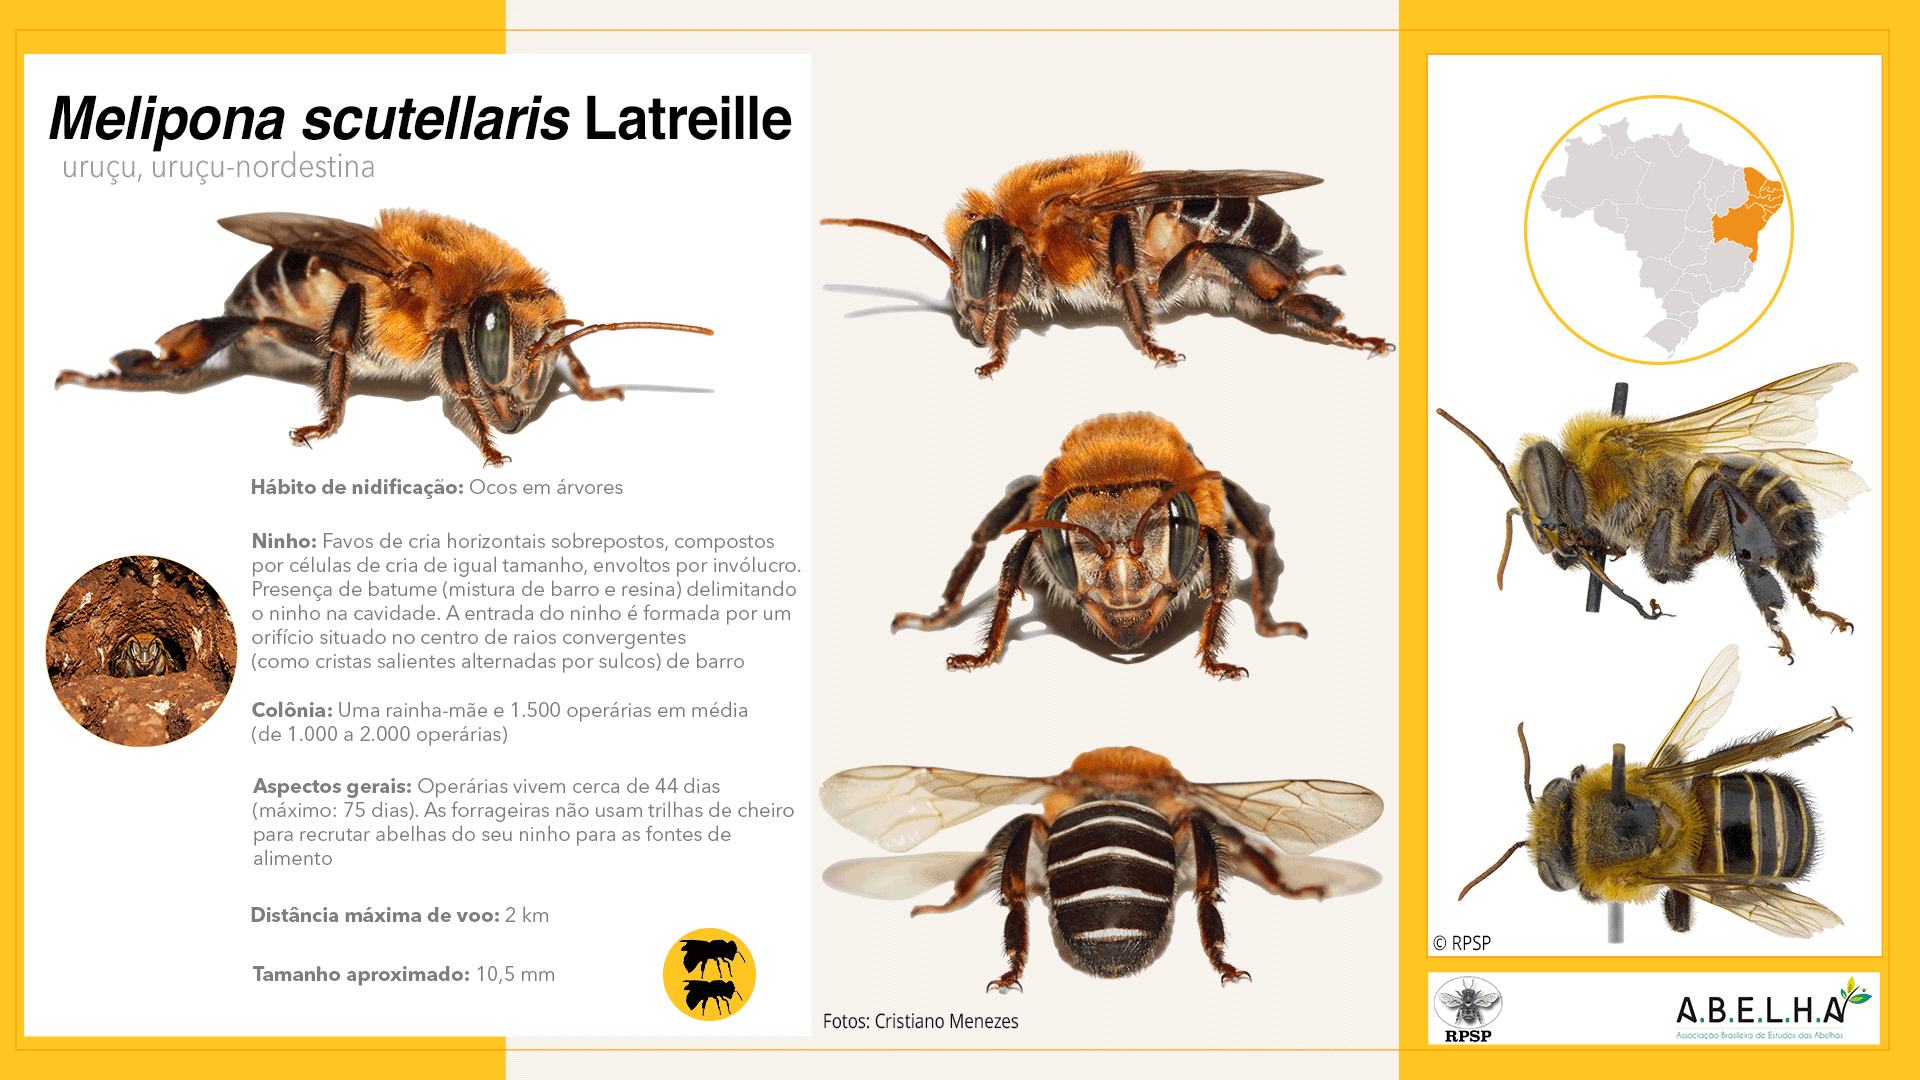
\includegraphics[width=0.83\textwidth]{figuras/Trabalhos Correlatos/Melipona-scutellaris.png}
     \fonte{\citeonline{menezes2022fichasMeliponicultura}}%% Fonte
 \end{figure}
 
\section{Trabalhos Relacionados}
O presente projeto articula três áreas principais de conhecimento: a meliponicultura, os Modelos de Distribuição de Espécies (\gls{sdm}) e o Processamento Digital de Imagens. Esta seção pretende apresentar os principais trabalhos da literatura relacionados a cada um desses eixos temáticos, destacando abordagens, metodologias e resultados relevantes que fundamentam e orientam o desenvolvimento desta pesquisa.

\subsection{Aplicações e projetos de incentivo à meliponicultura}
Para o incentivo da prática de meliponicultura, a A.B.E.L.H.A desenvolveu um aplicativo \footnote{Disponível em https://abelha.org.br/abelha-app-agora-disponivel-tambem-na-app-store/} para auxiliar no entendimento sobre o tema com artigos sobre mel, polinização e conservação das abelhas. Para os usuários já produtores, o aplicativo \textit{Beeh App} \footnote{Disponível em https://beeh.app/}, desenvolvido pela empresa homônima, propõe um sistema de controle de enxames para os meliponicultores, organizando datas de alimentação e para colheita. 

Esses projetos diferem do presente trabalho devido ao foco de desenvolvimento, visto que o aplicativo desenvolvido pela \textit{Beeh App} visa auxiliar pessoas que já praticam a meliponicultura e o sistema da A.B.E.L.H.A informa pessoas interessadas em iniciar a prática com artigos e imagens. O produto visado como resultado deste trabalho facilitará a escolha das abelhas, não somente com textos, mas também utilizando de tecnologias para entender quais as espécies adequadas para a região. 

Em Curitiba, a prefeitura criou o projeto ``Jardins de Mel'', que teve seu início no ano de 2018, visando conscientizar a população sobre a importância das abelhas sem ferrão. Para isso, foram espalhados 53 meliponários, com diferentes espécies, em parques da cidade. O trabalho de ensinar sobre os benefícios das melíponas também foi aplicado em escolas, o projeto ``AbeLinhas'' propôs uma extensão do ``Jardins de Mel'', apresentado em mais de 30 unidades de ensino como Centros Municipais de Educação Infantil (CMEI) e Escolas Municipais da cidade, promovendo o incentivo para as crianças pesquisarem sobre o assunto, além de serem instalados meliponários ao redor das unidades de ensino para que os alunos cuidassem e tivessem maior proximidade com os insetos \cite{abeLinhas:2019}.



\subsection{Modelos de Distribuição de Espécies}
Conforme apresentado na Seção \ref{sec:sdm}, o \gls{sdm} é uma técnica utilizada para prever a adaptabilidade de uma espécie em diferentes condições ecológicas. Essa modelagem pode ser realizada de diversas formas, conforme destacado por \citeonline{zhang:2017} em sua revisão sobre o tema.
Para este estudo, realizou-se uma busca na plataforma \textit{Google Scholar \footnote{https://scholar.google.com/}}, utilizando a expressão \textit{("Species Distribution Modeling" OR "Modelagem de Distribuição de Espécies")}, filtrando por trabalhos publicados a partir de 2024. Foram excluídos os trabalhos de revisão. A Tabela \ref{tab:usos_sdm} apresenta os diferentes objetivos de aplicação do \gls{sdm} identificados na amostra analisada.

\begin{table}[h]
 \captionsetup{width=0.83\textwidth}
 \centering
 \caption{Usos do SDM e respectivas referências}\label{tab:usos_sdm}
\begin{tabular}{p{8cm} c}
\toprule
\textbf{Uso do SDM} & \textbf{Referências bibliográficas} \\
\midrule
\textbf{Análise de distribuição potencial da espécie }
&\cite{Carlos:2025}\\
&\cite{Abadijoo2025}\\
&\cite{Zhang_He_Hui_Sha_Cheng_2025}\\
&\cite{radovi:2025}\\
&\cite{Song_Xu_Long_Wang_Chen_Li_Jiang_Deng_2024}\\
&\cite{Vaishnav_Maurya_Durgapal_Rana_2025}\\
&\cite{Sheidai_Noormohammadi_Alishah_2024}\\
&\cite{Singleton:2024}\\
&\cite{gutierrez:2024}\\
&\cite{han_2024}\\
&\cite{Oskolski_2024}\\
&\cite{Edalat_2025}\\
&\cite{zhao:2024}\\
&\cite{wang:2024}\\
\midrule
\textbf{Estratégias de conservação}
  & \cite{Tao_Liu_Dao_Liu_Yang_Sun_2024} \\
  & \cite{Adjacou_Idohou_Yaoitcha_Ayena_Houehanou_Gouwakinnou_2025} \\
\midrule
\textbf{Impacto de invasores}
  & \cite{Ruzzier_Lupi_Tirozzi_Dondina_Orioli_Jucker_Bani_2024} \\
  & \cite{Abadijoo2025} \\
\midrule
\textbf{Impacto das mudanças climáticas}
  & \cite{Ruzzier_Lupi_Tirozzi_Dondina_Orioli_Jucker_Bani_2024} \\
  & \cite{Dogbo_2025} \\
  & \cite{Habibi_Achour_Bounaceur_Benaradj_Aulagnier_2024} \\
\midrule
\textbf{Mapeamento de habitat}
  & \cite{Overly_Lecours_2024} \\
  & \cite{Zenebe_2024} \\
\bottomrule
\end{tabular}
 \fonte{Produção Própria}
\end{table}

Entre os 21 artigos analisados, dez tratavam de espécies de plantas, dez de espécies de animais e um abrangia ambos os reinos. Observa-se que nenhum deles abordou especificamente abelhas da tribo \textit{Meliponini}, diferindo, portanto, da proposta deste trabalho.

No que se refere à aplicação de modelos, \citeonline{zhang:2017} apresentam em sua revisão diferentes abordagens possíveis. De forma semelhante, \citeonline{beery_cole_parker_perona_winner_2021} destacam o \textit{BIOCLIM} como o primeiro algoritmo desenvolvido para a prática de \gls{sdm}. Atualmente, outros métodos são amplamente empregados, como o \gls{maxent} \cite{BRANCO2023110091}, o \gls{svm} \cite{miyaji_2024} e o \gls{garp} \cite{illoldi:2008}.

\subsection{Processamento Digital de Imagens}
O termo \gls{pdi} refere-se à análise e manipulação de imagens, visando melhorar suas características e/ou extrair informações relevantes \cite{costa:1998}. O \gls{pdi} possui diversas aplicações em outras áreas do conhecimento, como medicina \cite{Schiabel:2019}, engenharia civil \cite{Vital_Ferreira_2024}, agricultura \cite{silva2024identificacao}, entre outras. 
Imagens de satélite são comumente utilizadas por autores da área de \gls{sdm} \cite{beery_cole_parker_perona_winner_2021}, para obter índices ecológicos para analisar a distribuição de espécies. No entanto, há diferentes satélites disponíveis para esses fins, e os pesquisadores podem escolher entre eles de acordo com a aplicação desejada.
Para compreender o panorama atual do uso de satélites em estudos de \gls{sdm}, realizou-se uma busca na plataforma \textit{Google Scholar \footnote{https://scholar.google.com/}}, utilizando a seguinte expressão: \textit{(''SDM'' OR ''Species Distribution Modeling'' OR ''Modelagem de Distribuição de Espécies'') AND (''Landsat'' OR ''Modis'' OR ''Sentinel'' OR ''Satellite'' OR ''Satélite'')}. A pesquisa considerou apenas artigos publicados a partir do ano de 2024.
Os resultados incluíram artigos que mencionavam o termo \gls{sdm} (em português ou inglês) e, ao menos, um dos três principais satélites atualmente disponíveis para pesquisa, ou, alternativamente, a palavra ''satélite'', no caso de uso de outros sensores. A Tabela \ref{tab:satelites} apresenta os 17 artigos encontrados nas duas primeiras páginas da busca e considerados relevantes aos fundamentos da presente pesquisa. Já a Figura \ref{fig:satelites} ilustra a distribuição desses artigos agrupados por satélite utilizado.
Observa-se uma preferência pelo uso do satélite Sentinel, pertencente ao projeto \textit{Copernicus}\footnote{\url{https://browser.dataspace.copernicus.eu/}}. Por essa razão, o Sentinel-2 foi adotado neste projeto.

\begin{table}[h]
 \captionsetup{width=0.83\textwidth}
 \centering
 \caption{Satélites e suas aplicações em estudos acadêmicos}\label{tab:satelites}
\begin{tabular}{p{6cm} cccc}
\toprule
\textbf{Satélite} & \textbf{Referências bibliográficas} \\
\midrule
Sentinel 
  & \cite{wegner_2024} \\
  & \cite{vantiel2024multiscalemultimodalspeciesdistribution} \\
  & \cite{chen_peng_li_chen} \\
  & \cite{murray_2024} \\
  & \cite{picek:2024} \\
  & \cite{Oliveira_Bernardino_Vieira_Augusto_2025} \\
  & \cite{DeGiorgi2025} \\
  & \cite{Spondylidis_Giannoulaki_Machias_Batzakas_Topouzelis_2024} \\
\midrule
ALOS PALSAR 
  & \cite{Crispim-Mendes_Valerio_Marques_Pita_Godinho_Silva_2024} \\
\midrule
Landsat 
  & \cite{Picek_Botella_Servajean_Leblanc_Palard_Larcher_Deneu_Marcos_Bonnet_Joly_2024} \\
  & \cite{Crego:2024} \\
  & \cite{chen_peng_li_chen} \\
  & \cite{Gupta_Zuquim_Tuomisto_2024} \\
  & \cite{Giachello_Lefosse_Simoncini_Bonato_2025} \\
  & \cite{Cupiche-Herrera_Westwood_McLaren_2024} \\
  & \cite{Jefferys:2024} \\
\midrule
MODIS 
  & \cite{Abadijoo2025} \\
\bottomrule
\end{tabular}
 \fonte{Produção Própria}
\end{table}

 \begin{figure}[!htb]
     \caption{Distribuição de artigos agrupados pelo uso de satélite}
     \label{fig:satelites}
     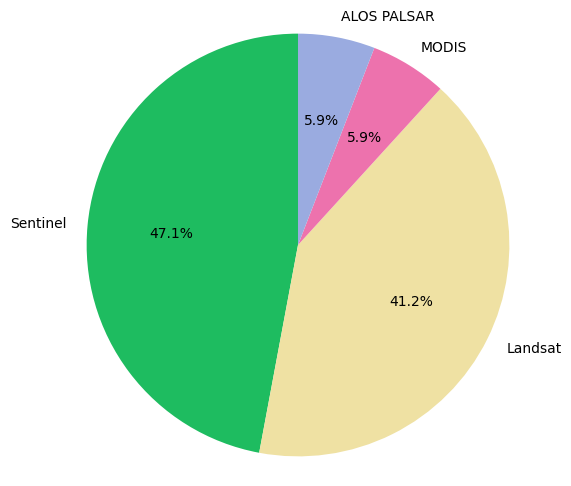
\includegraphics[width=0.5\textwidth]{figuras/Trabalhos Correlatos/satelites.png}
     \fonte{Produção Própria}%% Fonte
 \end{figure}

% ******************************

% Em relação ao assunto, o apresentado nesta seção pode estar relacionado a trabalhos de outros autores ou ao assunto que fornece a fundamentação (motivação) para o trabalho a ser desenvolvido. Se o assunto está relacionado a trabalhos de outros autores, a contribuição do trabalho é definida em relação ao que já foi pesquisado nesse assunto. Se o assunto será utilizado para embasamento do que será proposto, explicitar como o trabalho se insere nesse assunto. A contribuição pode, ainda, estar relacionada a uma necessidade de mercado ou a uma oportunidade decorrente de algum problema real para o qual se pretender propor uma solução. Nesse caso, o assunto fornece um contexto teórico de suporte para o problema e/ou a solução.

% O importante nesta seção é deixar claro do que se trata o trabalho (assunto ou tema), identificar o objeto de pesquisa, como será encaminhada a solução (procedimento metodológico, tecnologias, ferramentas utilizadas) e o que se pretende ao final do trabalho, sem explicitar a solução e os resultados.

% \caixa{Atenção}{As seções a seguir são sugestões, converse com o seu orientador para ver quais seções devem ter em seu trabalho!}

% \begin{photograph}[!htb]%% Ambiente figure
%     %\captionsetup{width=0.55\textwidth}%% Largura da legenda
%     \caption{Exemplo de fotografia}%% Legenda
%     \label{fig:exemplo1}%% Rótulo
%     \includegraphics[scale=0.4]{foto1}%% Dimensões e localização
%     \fonte{Autoria Própria}%% Fonte
%     \addcontentsline{loge}{photograph}{\protect\numberline{\thephotograph}Exemplo de fotografia.} % Adiciona à lista de ilustrações
% \end{photograph}


% \section{Objetivos}\label{sec:objetivos}

% Um texto curto\footnote{Teste de nota de rodapé 1.} apresentando a seção.



% \section{Objetivos específicos (opcional)}\label{subsec:objetivosEspecificos}

% Os objetivos específicos são opcionais, ou seja, somente devem ser apresentados se caracterizarem resultados parciais gerados a partir do objetivo geral, os quais sejam considerados úteis para a comunidade acadêmica, para a sociedade ou para o ambiente profissional. Uma observação importante é que os resultados sejam passíveis de comprovação, ou seja, se o objetivo for: “Oferecer agilidade e confiabilidade aos processos gerenciais da empresa”, significa que o trabalho deverá realizar testes com relação a esses atributos, cujos resultados deverão ser apresentados nas discussões do trabalho.

% \begin{graph}[!htb]%% Ambiente figure
%     %\captionsetup{width=0.55\textwidth}%% Largura da legenda
%     \caption{Exemplo de gráfico}%% Legenda
%     \label{graph1}%% Rótulo
%     \includegraphics[scale=0.4]{grafico2}%% Dimensões e localização
%     \fonte{Adaptado de \citeonline[p.~4]{UTFPR2008}}%% Fonte
%     \addcontentsline{loge}{graph}{\protect\numberline{\thegraph}Exemplo de gráfico.}
% \end{graph}


% Destaca-se que os objetivos específicos não incluem as etapas do processo de desenvolvimento de software (realizar a modelagem, a análise, o projeto...) ou outras atividades necessárias para alcançar o objetivo geral, como, estudar as tecnologias necessárias para modelagem e implementação do sistema. Dentre as exceções estão a realização de estudos, procedimentos, métodos e técnicas considerados inéditos e de relevância para outros trabalhos a serem realizados na mesma área. Contudo, o resultado deste estudo deve ser documentado de forma que seja conhecimento disponibilizado para quem lê o trabalho.


% \section{Justificativa}\label{sec:justificativa}

% Justificar o objeto de pesquisa (o que será feito) e a forma de resolução do problema (como fazer). A forma de resolução pode estar centrada no método, nas tecnologias, no uso de conceitos (fundamentação teórica).

% A Justificativa explicita porque desenvolver o referido trabalho, como o mesmo se insere no contexto de pesquisa, de produção científica. Pode incluir o porquê utilizar as tecnologias e ferramentas indicadas, a contribuição em termos de inovação ou mesmo de aprendizado.

% O trabalho não precisa ser justificado em decorrência de ser inovador ou por ter gerado uma significativa contribuição ao conhecimento na área em que o mesmo se insere. Pode referir-se simplesmente à aplicabilidade de conhecimentos adquiridos durante o curso. Sendo assim, a justificativa não deve ser elaborada considerando um mercado a ser atingido e sim com relação ao uso de tecnologias aprendidas e/ou estudadas, o conhecimento e aprendizado do aluno e a aplicabilidade do trabalho desenvolvido.

% \section{Estrutura do trabalho}\label{sec:estruturaTrabalho}

% A estrutura do trabalho contém uma relação dos capítulos e uma descrição sucinta do que cada um deles contém. Esta seção fornece uma visão geral do trabalho no sentido da sua estrutura em capítulos\footnote{Teste de nota de rodapé 2.}.

% \caixa{Atenção}{O OverLeaf está demorando muito para compilar o modelo com o Capítulo de Exemplos, que explica como usar o LaTeX. Assim, esse capítulo foi removido (está comentado para não compilar), mas há um arquivo chamado \texttt{exemploPDF.pdf}, na raiz do projeto, que contém esse capítulo de exemplos!}


